\documentclass[a4paper,12pt]{jarticle}
\input ./chap01_preamble.tex
\graphicspath{%
  {../text01-img/}%
}
% !TEX root = ./chap01_08.tex
\begin{document}
\section{質問フォーム}
わからないこと、質問したいことがあれば質問フォームから質問しよう!

質問フォームでは、授業でわからなかったことや確認したいことなどをホームページを通して質問できます。たくさん質問してわからないことを解決しよう。

1.
ブラウザで\textbf{授業で使うホームページリスト}を開こう。

\textbf{授業で使うホームページリスト}は01フォルダの中のlinks.htmlです

リストの4番目の子ども\textbf{IT未来塾質問フォーム}をクリックして開いてください(Figure~\ref{seq:refFigure46})。


\bigskip

{\bfseries
  スマートフォン等からの場合は\url{https://bit.ly/2NHiVgi}を開いてください。}



\centering
\begin{minipage}{\textwidth}
  {\upshape
    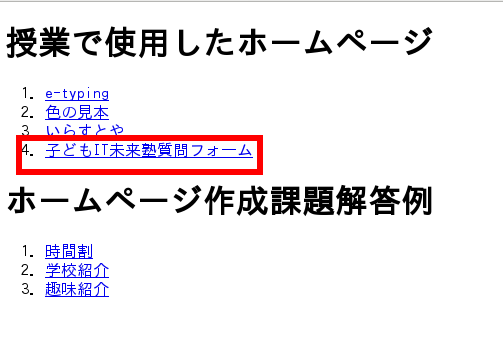
\includegraphics[width=0.9\textwidth]{textbook-img245.png}
    \flushleft

    \bigskip
    {\refstepcounter{Figure}\theFigure\label{seq:refFigure46}}:
    ホームページリストより質問フォームを開く}
\end{minipage}

\bigskip

\bigskip

2.
質問フォーム(~\ref{seq:refFigure47})が表示されます

\centering
\begin{minipage}{\textwidth}
  {\upshape
    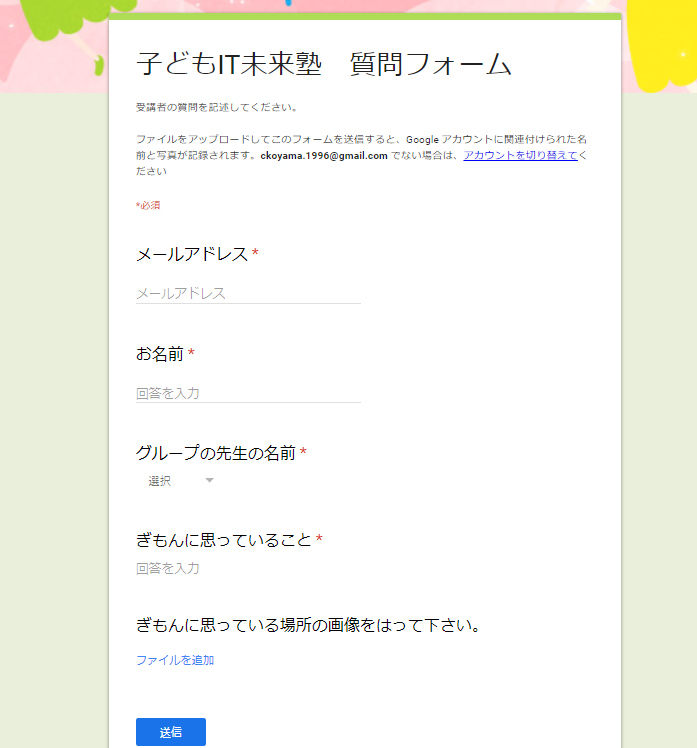
\includegraphics[width=0.8\textwidth]{textbook-img246.png}
    \flushleft

    \bigskip
    {\refstepcounter{Figure}\theFigure\label{seq:refFigure47}}: 質問フォーム}
\end{minipage}
\flushleft

\bigskip

メールアドレス、お名前、グループの先生の名前、ぎもんに思っていることを入力します。必要に応じて、ぎもんに思っている場所の画像を追加してください。

{\bfseries
送信\textmd{を押すと質問ができます。~\ref{seq:refFigure48}の画面が出たら質問は完了です。}}



\centering
\begin{minipage}{\textwidth}
  {\upshape
    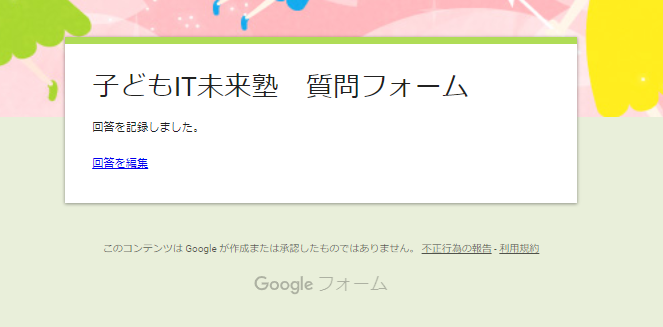
\includegraphics[width=0.45\textwidth]{textbook-img247.png}
    \flushleft

    \bigskip
    {\refstepcounter{Figure}\theFigure\label{seq:refFigure48}}: 質問送信画面}
\end{minipage}
\flushleft
メールアドレスのらんに入力したアドレスへグループの先生から回答メールがきます。
メールが来るまで、しばらくお待ちください。数日かかる場合があります。
\end{document}
